\documentclass[11pt]{article}
%%%%%%%%%%%%%%%%%%%%%%%%%%%%%%%%%%%%%%%%
\usepackage[utf8x]{inputenc}
\usepackage{lmodern}
\usepackage[T1]{fontenc}
%%%%%%%%%%%%%%%%%%%%%%%%%%%%%%%%%%%%%%%%
\usepackage[dvipsnames]{xcolor}
\usepackage{graphicx}
\usepackage{caption}
\usepackage{amsmath, amssymb, amsfonts}
\usepackage{layout}
\usepackage{txfonts}
\usepackage{geometry}
\usepackage[round]{natbib}
\bibliographystyle{plainnat}
\geometry{a4paper,left=15mm,right=10mm, top=1cm, bottom=1.4cm}
\usepackage{float}
\usepackage{listings}
\usepackage[colorlinks=true, allcolors=Blue]{hyperref}
\usepackage{caption}
\usepackage{booktabs} %allows for short midlines
%\usepackage{subcaption}
%%%%%%%%%%%%%%%%%%%%%%%%%%%%%%%%%%%%%%%%
\title{Bonustoets examen vragen}


\begin{document}

\title{Bonustoets ANI}


\section{Oefening 1}
Een kogel met een massa $m_1$ wordt in een horizontale richting afgeschoten naar een zwaar blok met massa $M_2$. Dit zware blok is bevestigd aan een gefixeerde horizontale veer met een veerconstante $k$.
De kogel blijft na inslag vastzitten in de blok en zorgt ervoor dat de blok (met kogel in) aan de veer een horizontale trilling ondergaat.\\
Geef een uitdrukking voor de horizontale beginsnelheid van de kogel, die ervoor zorgt dat het blok een trilling met amplitude $\Delta x = A$ ondergaat, in functie van $m_1$, $M_2$, $A$ en $k$.\\
Je mag het effect van versnellingen door zwaartekracht of weerstand op de kogel tijdens het schot verwaarlozen.


\subsection{Oplossing}
Behoud van impuls tijdens botsing, en behoud van energie: van kinetische energie van het blok + kogel naar elastische energie van de veer bij maximale amplitude.

Behoud van energie:
\begin{equation}
 	\frac{1}{2}  v_{\rm b+k}^{2} (m+M) = \frac{1}{2} k A^2
\end{equation}
waaruit je kan halen dat
\begin{equation}
	v_{\rm b+k} = A \left(\frac{k}{m+M}\right)^{1/2}
\end{equation}

Behoud van impuls:
\begin{equation}
	mv_0 = (m+M) \cdot v_{\rm b+k}
\end{equation}
waaruit volgt:
\begin{equation}
	v_0 = \frac{\sqrt{(m+M) \cdot k}}{m} A
\end{equation}

\section{Oefening 2}
Een boot vaart met een snelheid $v$ op water indien er geen stroming is.
Stel dat er op de rivier een stroming $u$ zit (evenwijdig met de oever), en de boot een kleine rondvaart wil doen waarin hij een totale afstand $D$ af legt (heen en terug samen). Wat is dan een uitdrukking voor de totale tijd $t$ die de boot nodig heeft voor zijn rondvaart in volgende 2 situaties:

\begin{itemize}
	\item De boot vaart eerst tegen de stroom in en keert terug met de stroom mee.
	\item Iemand die op de oever staat ziet de boot varen in een rechte lijn loodrecht op de oever naar de overkant en terug.
\end{itemize}

\subsection{Oplossing}
Zoek de snelheid van de boot ten opzichte van de oever via $\vec{v'}= \vec{v} + \vec{u}$ voor heen en terug, en bepaal de tijd apart voor heen en terug via $t' = \frac{D/2}{v'}$.

\begin{itemize}
	\item $t_1 = \frac{D/2}{v-u}$, $t_2 = \frac{D/2}{v+u}$, so $t=\frac{Dv}{(v^2 - u^2)}$
	\item $v' = \sqrt{v^2 - u^2}$, so $t_1 = t_2 = \frac{D/2}{\sqrt{v^2 - u^2}}$, so $t = \frac{D}{\sqrt{v^2 - u^2}}$
\end{itemize}

\section{Oefening 3}
Een vlakke hockey puck met massa M ligt op een air hockey tafel zodat er geen wrijving is.
De puck beweegt in een cirkel met constante straal op deze tafel omdat het aan een touw hangt dat door een opening in de tafel loopt.
Aan de andere kant van het touw hangt een gewicht met massa $m$ die het touw strak houdt.
Toon aan dat de snelheid van de puck gegeven wordt door: $v = \sqrt{\frac{mgR}{M}}$ waar $R$ de afstand is tussen de puck en de opening in de tafel.

\begin{figure}
\centering
	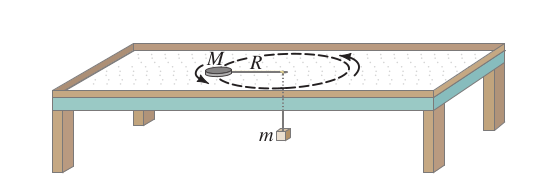
\includegraphics[width=0.6\textwidth]{hockeypuck}
	\caption{}
	\label{fig:hockeypuck}
\end{figure}

\subsection{Oplossing}

De spankracht op het gewicht onder tafel is $F_T = mg$. Dit moet gelijk zijn aan de spankracht op de hockey puck.
Dit is de enige kracht die werkt op de puck en is de oorzaak voor de rotatie. Gebruik dit samen met het feit dat dit een ECB is om te berekenen dat:
\begin{align}
	F_T = mg &= M \frac{Mv^2}{R}\\
	v &= \sqrt{\frac{mgR}{M}}
\end{align}
\section{Oefening 4}
Ingenieurs zijn een achtbaan aan het ontwikkelen. Het is een simpel ontwerp waarbij een karretje van massa $M$ eerst naar een hoogte $h$ wordt getild, dan losgelaten wordt en daarna een (cirkelvormige) looping van radius $R$ doorgaat. Neem aan dat er geen wrijving is.
\begin{itemize}
	\item Wat is de minimale hoogte $h$ als functie van $R$ en $M$ zodanig dat het karretje zonder problemen door de looping gaat?
	\item Als er mensen in het karretje gaan zitten, moeten de ingenieurs dan rekening houden met de massa van die mensen? Zo ja, zal dat gewicht ervoor zorgen dat je het karretje hoger moet tillen of net lager?
\end{itemize}
\subsection{Oplossing}
We berekenen eerst de snelheid $v$ bovenaan de looping in functie van de hoogte met behulp van behoud van energie.
\begin{align}
	mg h&=2mgR+\frac{m v^2}{2}\\
	g h&=2gR+\frac{ v^2}{2}\\
	v^2&=2g(h-2R).
\end{align}
Bovenaan in de looping werken er in principe twee krachten in in het systeem, een normaalkracht $-N \hat{j}$ en een zwaartekracht $-mg\hat{j}$. Aangezien de looping cirkelvormig is moet het karretje een centripetaal versnelling in de $-\hat{j}$ righting hebben. De grote van deze versnelling is
\begin{equation}
	a_{\text{cp}}=\omega^2R=\left(\frac{v}{R}\right)^2 R.
\end{equation}
Als we nu beide krachten en de versnelling in $\vec{F}=m\vec{a}$ invullen krijgen we
\begin{equation}
	m\frac{v^2}{R}=N+mg.
\end{equation}
De looping kan natuurlijk enkel een neerwaardse normaalkracht uitoefenen op het karretje en dus krijgen we
\begin{align}
	m\frac{v^2}{R}&\geq mg\\
	\frac{v^2}{R}&\geq g.
\end{align}
Het invullen van de bovenstaande vergelijking geeft nu
\begin{align}
	2(h-2R)&\geq R \\
	h&\geq \frac{5}{2}R.
\end{align}
Antwoord op de tweede deelvraag het maakt dus niet uit hoeveel de passagiers wegen (dat is natuurlijk enkel zo omdat we de wrijvingskrachten negeerden).
\end{document}
